% file: compatible-paths.tex

\documentclass[tikz]{standalone}

\usepackage{amssymb}
\usetikzlibrary{shapes, positioning, arrows.meta, calc, backgrounds, fit, decorations.pathmorphing}

\newcommand{\state}[3]{% #1: state name; #2: position; #3: state label
  \node (#1) [circle, inner sep = 0pt, minimum size = 8mm, text width = 8mm, align = center, draw, #2, font = \Large] {#3};
}

\tikzset{every edge/.style = {draw, >=Stealth, ->, decorate, decoration = {snake, post length = 1mm}}}

\begin{document}
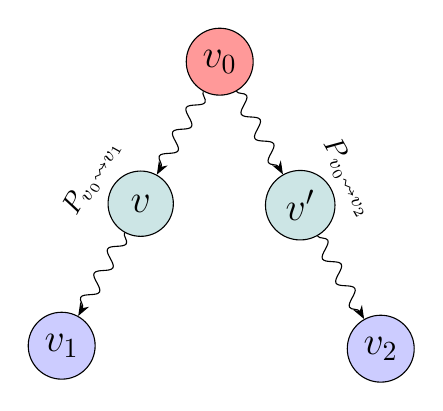
\begin{tikzpicture}[node distance = 1.2cm and 0.4cm]
  \state{0}{fill = red!40}{$v_0$};

  \state{v}{fill = teal!20, below left = of 0}{$v$};
  \state{v'}{fill = teal!20, below right = of 0}{$v'$};

  \state{1}{fill = blue!20, below left = of v}{$v_1$};
  \state{2}{fill = blue!20, below right = of v'}{$v_2$};

  \path (0) edge (v)
  	    edge (v')
  	(v)  edge (1)
	(v') edge (2)
	(0)  edge[draw = none] node[sloped, above = 12pt] {$P_{v_0 \leadsto v_1}$} (1)
	(0) edge[draw = none] node[sloped, above = 12pt] {$P_{v_0 \leadsto v_2}$} (2);
\end{tikzpicture}
\end{document}
